\documentclass[12pt]{ociamthesis}  %  UPC logo
%%%%%%%%%%%%%%%%%%%%%%%%%%%%%%%%%%%%%%%%%% Disclaimer %%%%%%%%%%%%%%%%%%%%%%%%%%%%%%%%%%%%%%%%%%%%
%This is not an official UPC template. I gathered the resources for my personal use. And I'm happy to share it with anyone who wants to use something out-of-the-box BS/Master/Ph.D latex template. This is a template that based on Oxford/Cambridge LaTeX Phd thesis template with ACL/CVPR confer template inspired modification. 
% original temp github
%https://github.com/mcmanigle/OxThesis
% this temp gitgub
%https://github.com/sabirdvd/LaTeX-template-for-UPC-thesis-
%%%%%%%%%%%%%%%%%%%%%%%%%%%%%%%%%%%%%%%%%% Disclaimer %%%%%%%%%%%%%%%%%%%%%%%%%%%%%%%%%%%%%%%%%%%%

%load any additional packages
\usepackage{amssymb}
\usepackage{graphicx,pstricks}
\usepackage{graphics}
\usepackage{moreverb}
\usepackage{subfigure}
\usepackage{epsfig}
\usepackage{subfigure}
\usepackage{lipsum}  
\usepackage{ragged2e}
\usepackage{hangcaption}
%\usepackage{txfonts}
\usepackage{palatino}
%\usepackage[table]{xcolor}
\usepackage{color}
\usepackage{graphicx}
\usepackage{amsmath,amssymb} % define this before the line numbering.
%\usepackage{ruler}
\usepackage[noend]{algpseudocode}
\usepackage{amsmath,amssymb} % define this before the line numbering.
%\usepackage{ruler}
\usepackage{color}
\usepackage{comment}
\usepackage{bm,nicefrac} % bold math package
\usepackage{amsmath}
\usepackage{tikz}
\DeclareMathOperator*{\argmax}{argmax}
\usepackage{hyperref}
\usepackage{color}
\usepackage{threeparttable}
\usepackage[linesnumbered, ruled]{algorithm2e}
\SetKwRepeat{Do}{do}{while}
\usepackage{graphicx}
\usepackage{color,soul}
%\usepackage{fancyhdr}
%\setlength{\headheight}{15pt}
%\pagestyle{fancy}
%\renewcommand{\chaptermark}[1]{\markboth{#1}{}}
%\renewcommand{\sectionmark}[1]{\markright{#1}{}}
\definecolor{ao}{rgb}{0.0, 0.5, 0.0}

\usepackage{xcolor}
\usepackage{soul}

\newcommand{\hlc}[2][yellow]{{%
    \colorlet{foo}{#1}%
    \sethlcolor{foo}\hl{#2}}%
}


\usepackage{amsmath}
\DontPrintSemicolon
%\usepackage{algorithm}
%\usepackage[linesnumbered,ruled]{algorithm2e}
\usepackage[noend]{algpseudocode}
\usepackage{amsmath,amssymb} % define this before the line numbering.
%\usepackage{ruler}
\usepackage{color}
\usepackage{xcolor}
\definecolor{darkblue}{rgb}{0, 0, 0.5} 
\usepackage{amsmath}
%\DeclareMathOperator*{\argmax}{argmax}
\definecolor{bluegray}{rgb}{0.4, 0.6, 0.8}
\usepackage{hyperref}

%%%%%%%%%%%%%%%%%% Gray box %%%%%%%%%%%%%%%
\usepackage[breakable, theorems, skins]{tcolorbox}
\DeclareRobustCommand{\mybox}[2][gray!20]{%
\begin{tcolorbox}[   %% Adjust the following parameters at will.
        breakable,
        left=0pt,
        right=0pt,
        top=0pt,
        bottom=0pt,
        colback=#1,
        colframe=#1,
        width=\dimexpr\textwidth\relax, 
        enlarge left by=0mm,
        boxsep=5pt,
        arc=0pt,outer arc=0pt,
        ]
        #2
\end{tcolorbox}
}


%

\hypersetup{
  colorlinks   = true, %Colours links instead of ugly boxes
  urlcolor     = black, %Colour for external hyperlinks
  linkcolor    = red, %Colour of internal links RoyalBlue
   % linkcolor    = violet, %Colour of internal links RoyalBlue
   %linkcolor    =  bluegray, %Colour of internal links
  %citecolor   = red %Colour of citations
  %citecolor = blue %black darkblue
  citecolor = darkblue
}
%{ \hypersetup{hidelinks} \tableofcontents }

\hypersetup{linktoc = all}
\hypersetup{linktoc = page} 

\usepackage{lineno,hyperref}
\usepackage{caption} 
\captionsetup[table]{skip=10pt}
\usepackage{color}
\usepackage{graphicx}
\usepackage{amsmath,amssymb} % define this before the line numbering.
%\usepackage{ruler}
\usepackage{color}
\usepackage{threeparttable}
%\usepackage[linesnumbered, ruled]{algorithm2e}
\modulolinenumbers[4]
\usepackage[noend]{algpseudocode}
\usepackage{amsmath,amssymb} % define this before the line numbering.
%\usepackage{ruler}
\usepackage{color}
\usepackage{comment}
\usepackage{bm,nicefrac} % bold math package
\usepackage{amsmath}
\usepackage{tikz}
\usepackage{CJKutf8}
\usepackage{natbib}
\bibpunct{(}{)}{,}{a}{}{;}
\bibliographystyle{abbrvnat}
\renewcommand{\citep}[1]{[\citealp{#1}]}
%\DeclareMathOperator*{\argmax}{argmax}
\usepackage{hyperref}
\usepackage[english]{babel}
\usepackage[utf8]{inputenc}
\usepackage{fancyhdr}
\usepackage{enumitem} 
\usepackage[page,toc,titletoc,title]{appendix}
\usepackage{comment}
%%%%%%%%%%%%%%%%%%%%%%%%%%%%%
%\usepackage{xcolor}
%\usepackage{soulpos}
%\ulposdef{\hlc}[xoffset=1pt]{\mbox{\color{cyan!30}\rule[-.8ex]{\ulwidth}{3ex}}}
%%%%%%%%%%%%%%%%%%%%
\pagestyle{fancy}
\renewcommand{\chaptermark}[1]{\markboth{#1}{#1}}
\fancyhead[R]{}
\fancyhead[L]{\chaptername\ \thechapter\ --\ \leftmark}

\newcommand{\bert}{\ensuremath{%
  \mathchoice{\includegraphics[height=2ex]{Figure-Ch5/Bert.png}} 
    {\includegraphics[height=2ex]{Figure-Ch5/Bert.png}}
    {\includegraphics[height=1.5ex]{Figure-Ch5/Bert.png}}
    {\includegraphics[height=1ex]{Figure-Ch5/Bert.png}}
}} 


\pagestyle{fancy}
\fancyhf{}
\fancyhead[L]{\rightmark}
\fancyhead[R]{\thepage}
%\renewcommand{\headrulewidth}{0pt}
%%%%%%%%%%%%%%%%%%%%%%%%%% from CVPR %%%%%%%%%%%%%%%%%
\makeatletter
\DeclareRobustCommand\onedot{\futurelet\@let@token\@onedot}
\def\@onedot{\ifx\@let@token.\else.\null\fi\xspace}

\def\eg{\emph{e.g}\onedot} \def\Eg{\emph{E.g}\onedot}
\def\eg{\emph{e.g}\onedot} \def\Eg{\emph{E.g}\onedot}
\def\ie{\emph{i.e}\onedot} \def\Ie{\emph{I.e}\onedot}
\def\cf{\emph{c.f}\onedot} \def\Cf{\emph{C.f}\onedot}
\def\etc{\emph{etc}\onedot} \def\vs{\emph{vs}\onedot}
\def\wrt{w.r.t\onedot} \def\dof{d.o.f\onedot}
\def\etal{\emph{et al}\onedot}
%%%%%%%%%%%%%%%%%%%%%%%%%%CVPR %%%%%%%%%%%%%%%%%


%input macros (i.e. write your own macros file called mymacros.tex 
%and uncomment the next line)
%\include{mymacros}


\title{Mechanics of epithelial layers subjected to controlled pressure} 
\author{Nimesh Ramesh Chahare}

%\college{ {\larger \textit{By}  \vspace{0.3cm} \\ your name} \\  \vspace{0.1cm} Departament de Ci\`{e}ncies de la Computaci\'{o} }

%\renewcommand{\submittedtext}{change the default text here if needed}
\degree{Doctor of Philosophy \\ PhD Program in Applied Mathematics }     %the degree
\degreedate{Barcelona, April 2023}     

   
%end the preamble and start the document
\begin{document}

%this baselineskip gives sufficient line spacing for an examiner to easily
%markup the thesis with comments
\baselineskip=18pt plus1pt

%set the number of sectioning levels that get number and appear in the contents
\setcounter{secnumdepth}{3}
\setcounter{tocdepth}{3}


\maketitle                  % create a title page from the preamble info
\begin{dedication}

\begin{quote}
``You cannot carry out fundamental change without a certain amount of
madness. In this case, it comes from nonconformity, the courage to turn
your back on the old formulas, the courage to invent the future. It took
the madmen of yesterday for us to be able to act with extreme clarity
today. I want to be one of those madmen. We must dare to \textbf{invent the
future}.''\\
 - Thomas Sankara
\end{quote}

\end{dedication}
        % include a dedication.tex file
\begin{acknowledgements}
I would like to thank all the working people of the world
\end{acknowledgements}
   % include an acknowledgements.tex file
\begin{abstract}
Epithelial sheets are active viscoelastic materials that form
specialized 3D structures suited to their physiological roles, such as
branched alveoli in the lungs, tubes in the kidney, and villi in the
intestine. The shape of these structures depends on active stresses
generated by the actomyosin cytoskeleton, active viscoelastic properties
of the epithelium, and hydraulics of the luminal fluid. How these active
stress and material properties are linked to give rise to epithelial
shape remains largely unknown. Here we developed a new experimental and
computational approach to probe active epithelial viscoelasticity and
then harness the resulting constitutive relation to sculpt epithelia of
controlled 3D shape. We developed a microfluidic setup to engineer 3D
epithelial tissues with controlled shape and pressure. In this setup, an
epithelial monolayer is grown on a porous surface with circular low
adhesion zones (footprint). On applying hydrostatic pressure, the
monolayer delaminates into a spherical cap (dome) from the circular
footprint. Through this approach, we subject MDCK epithelial cells to a
range of lumen pressures at different rates and hence probe the relation
between strain and tension in different regimes. Slow pressure changes
relative to the timescales of actin dynamics allow the tissue to
accommodate large strain variations. However, under sudden pressure
reductions, the tissue develops buckling patterns and folds with
different degrees of symmetry-breaking to store excess tissue area. This
behavior is well captured by a 3D computational model that incorporates
the turnover, viscoelasticity and contractility of the actomyosin
cortex. Informed by this model, we harness the active behavior of the
cell cortex to pattern epithelial folds by rationally directed buckling.
Our study establishes a new approach for engineering epithelial
morphogenetic events.
\end{abstract}
          % include the abstract

\begin{romanpages}          % start roman page numbering
\tableofcontents            % generate and include a table of contents
\listoffigures              % generate and include a list of figures
\end{romanpages}            % end roman page numbering

%now include the files of latex for each of the chapters etc
\part{Introduction}


\hypertarget{introduction}{%
	\section{Introduction}\label{introduction}}

\begin{figure}[h!]
	\centering
	\includegraphics[width=0.7\textwidth]{chap1ruysch.png}
	\caption{\label{fig_1_1} \textbf{The Anatomy Lesson of Dr.~Frederik Ruysch}, 1670 by
		Adriaen Backer. \cite{ruyshc}}
\end{figure}

The term ``epithelia'' was first introduced by Dutch botanist Frederick Ruysch in the early 18th century (see fig \ref{fig_1_1}). He used it to describe the tissue he observed while dissecting the lips of a cadaver, and the word is derived from Greek roots ``epi,'' meaning top, and ``thele,'' meaning nipple.
\footnote{Ruysch is referred to as a ``Artist of death'' because of his famous anatomical collection. He was the first to use arterial embalming, which allowed for visualizing and dissecting smallest
	arteries. He also was part of the macabre practice of public dissections \cite{halley2019}.}
A few decades later, Swiss scientist Albrecht von Haller began using the term ``epithelium/epithelia'' to describe the fibers of the body, following the old Renaissance theory that the body was made of fibers, which were believed to be a fundamental building block of living things.
\footnote{Finding a fundamental unit of living entities comes from the philosophy of Gottfried W. Leibniz. It was based on the idea of ``monad''. Thanks to progress in microscopy and philosophy, naturalists were able to put together ideas for cells, fibers, and even cytoskeleton!\cite{zampieri2014}}
It was thought that these fibers and tissues arranged in different arrays gave rise to biological structures \cite{maccord2012, zampieri2014}. This theory was not far off, as epithelial tissues make up more than 60\% of the cells in a vertebrate's body and are found ubiquitously, covering the organs both inside and out \cite{alberts2015}.

\begin{wrapfigure}{r}{5cm}
	\caption{\textbf{Polarity of epithelia} Actin and myosin is distributed heterogenously in epithelial monolayers \cite{chen2018}.}\label{fig_1_2}
	\centering
	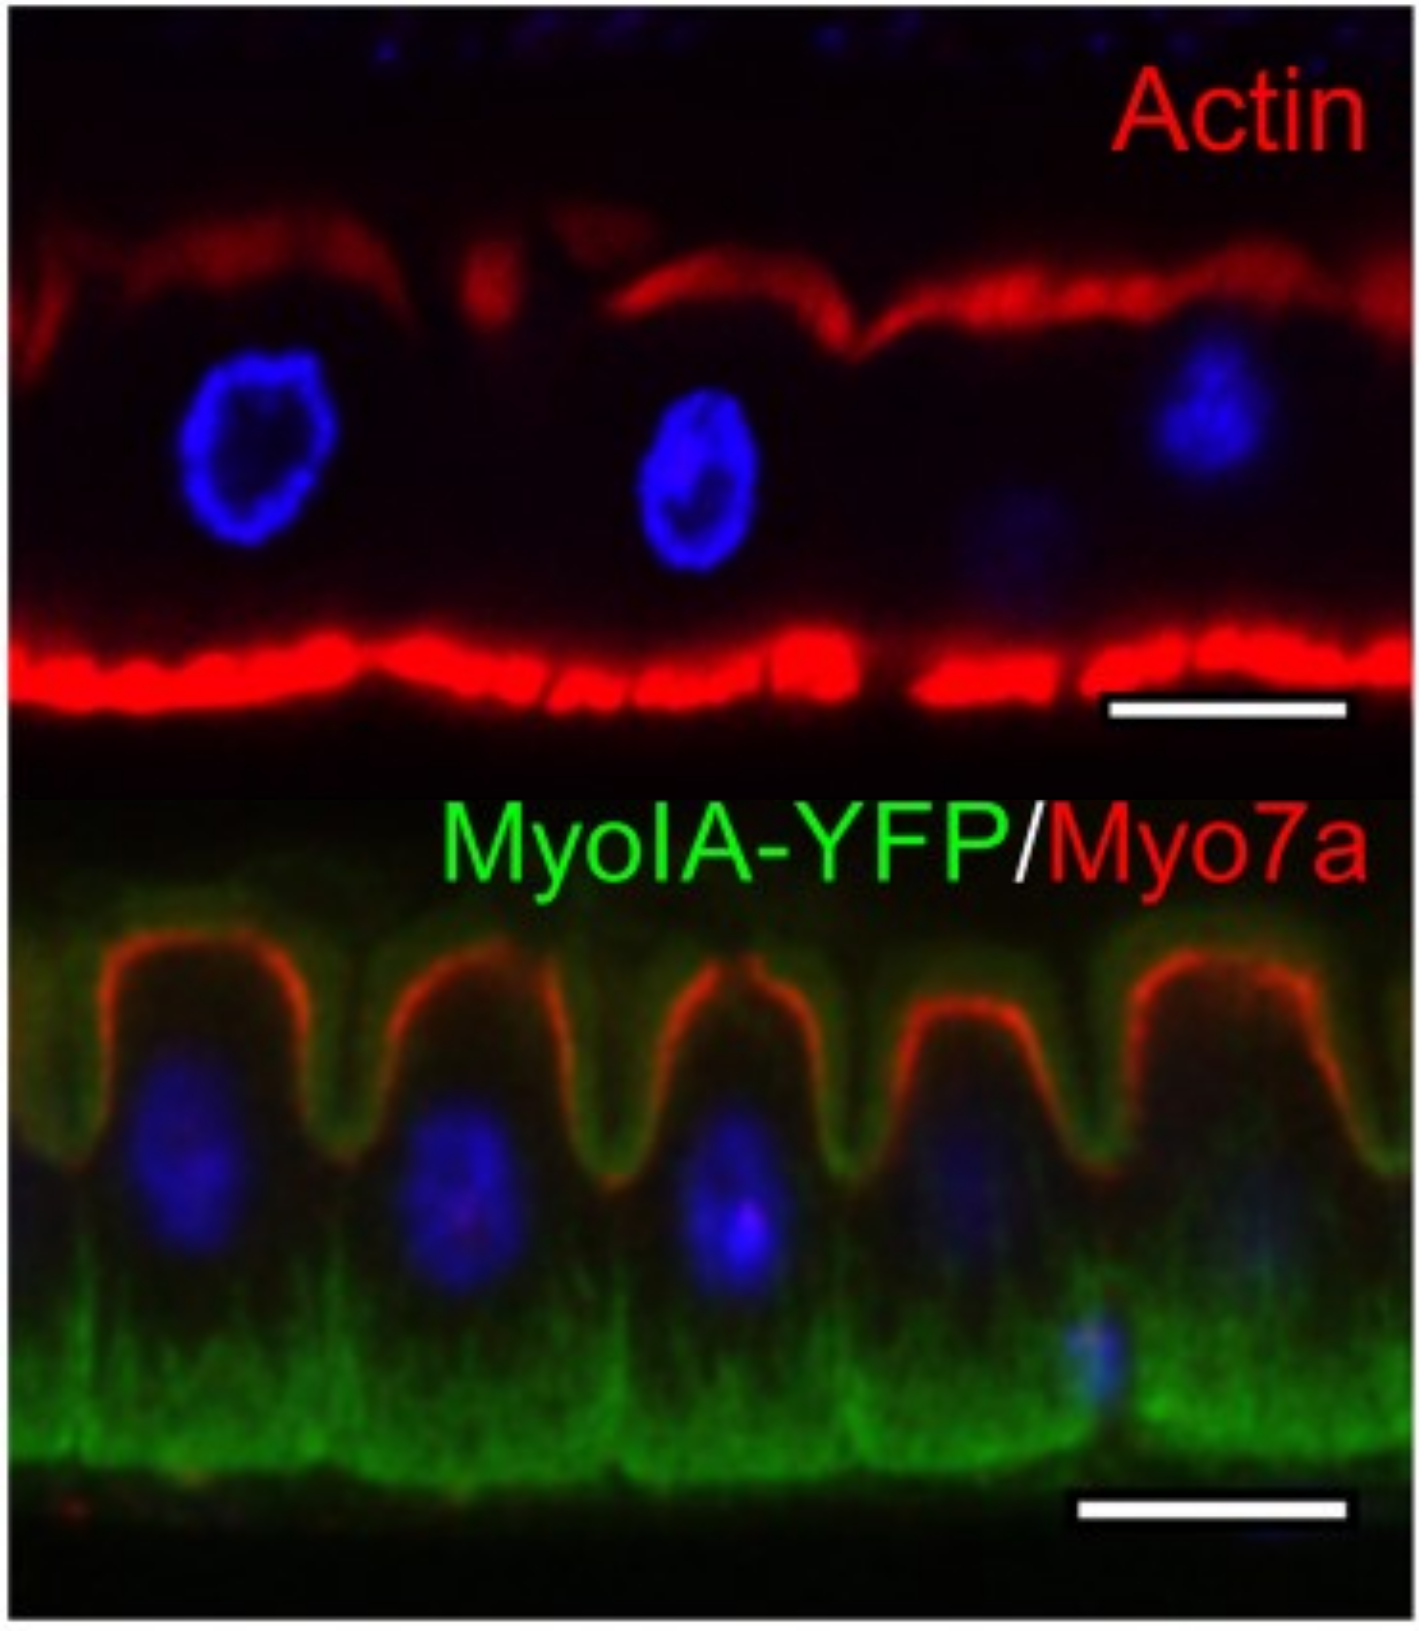
\includegraphics[width = 4cm]{chap1polarity.png}
\end{wrapfigure}

Epithelial cells are polarized, i.e., their apical side (typically facing the lumen of the organ), which differs in shape and composition from the basolateral side (see fig \ref{fig_1_2}). Its polar organization is reflected in the vectorial functions like creating and maintaining concentration gradients between separated compartments \cite{marchiando2010}. Typical examples of these are transporting epithelia such as those of the renal tubule, absorptive epithelia of the intestine, and secretory epithelial cells like hepatocytes \cite{alberts2015}. In addition, polarized epithelia guide the developmental process by determining the fate of cells leading to symmetry-breaking events in the embryo \cite{kim2018}.

\hypertarget{key-components}{%
	\section{Key components}\label{key-components}}

The function of epithelia primarily depends on the tissue's structure and the surrounding microenvironment. It can be divided into three aspects: cell structure, microenvironment, and cell-matrix interactions.

\hypertarget{cell-structure}{%
	\subsection{Cell structure}\label{cell-structure}}

The cell cytoskeleton plays a crucial role in maintaining cell shape and supporting vital functions such as cell division and migration \cite{alberts2015}. The Eukaryotic cell cytoskeleton is composed primarily of filamentous proteins, including three main types of filaments that differ in size and protein composition: microtubules, actin filaments, and intermediate filaments (see fig \ref{fig_1_3b}). Microtubules, with a diameter of approximately 25 nm, are the largest and made of the protein tubulin. Actin filaments, with a diameter of only 6 nm, are the smallest. Intermediate filaments, with a diameter of around 10 nm, are composed of several different subunit proteins and have a diameter intermediate between the other two types \cite{mofrad2009}. All three filament types dynamically respond to signals from the microenvironment and cell networks.

Mechanically, actin filaments have higher extensional stiffness than microtubules but break at lower extensions. Intermediate filaments have intermediate extensional stiffness and can sustain larger extensions while showing a nonlinear stiffening response \cite{wen2011}. Differences in strength and stability arise from the properties of individual subunits. The persistence length can range from 1\unit{\um} for intermediate filaments to 1\unit{\mm} for microtubules \cite{fletcher2010}. Actin filaments, most relevant to this thesis, have a persistence length of a few microns.

The assembly and disassembly of these filaments are dictated by the dynamics of their macromolecular components and accompanying proteins. The combination of actin filaments and myosin motors forms the actomyosin cortex, which is essential in producing intra- and intercellular forces. In an epithelial tissue, the actomyosin cortex and intercellular junctions make cell-to-cell contacts stronger and provide tissue integrity \cite{braga2016} (see fig \ref{fig_1_3}). A good example of these tissue-level structures can be observed in wound healing assays, where cells surrounding the wound create a ring of actin to close it \cite{brugues2014}. In Chapter 3, we will delve into the actomyosin network in more detail.

\begin{figure}[h!]
	\centering
	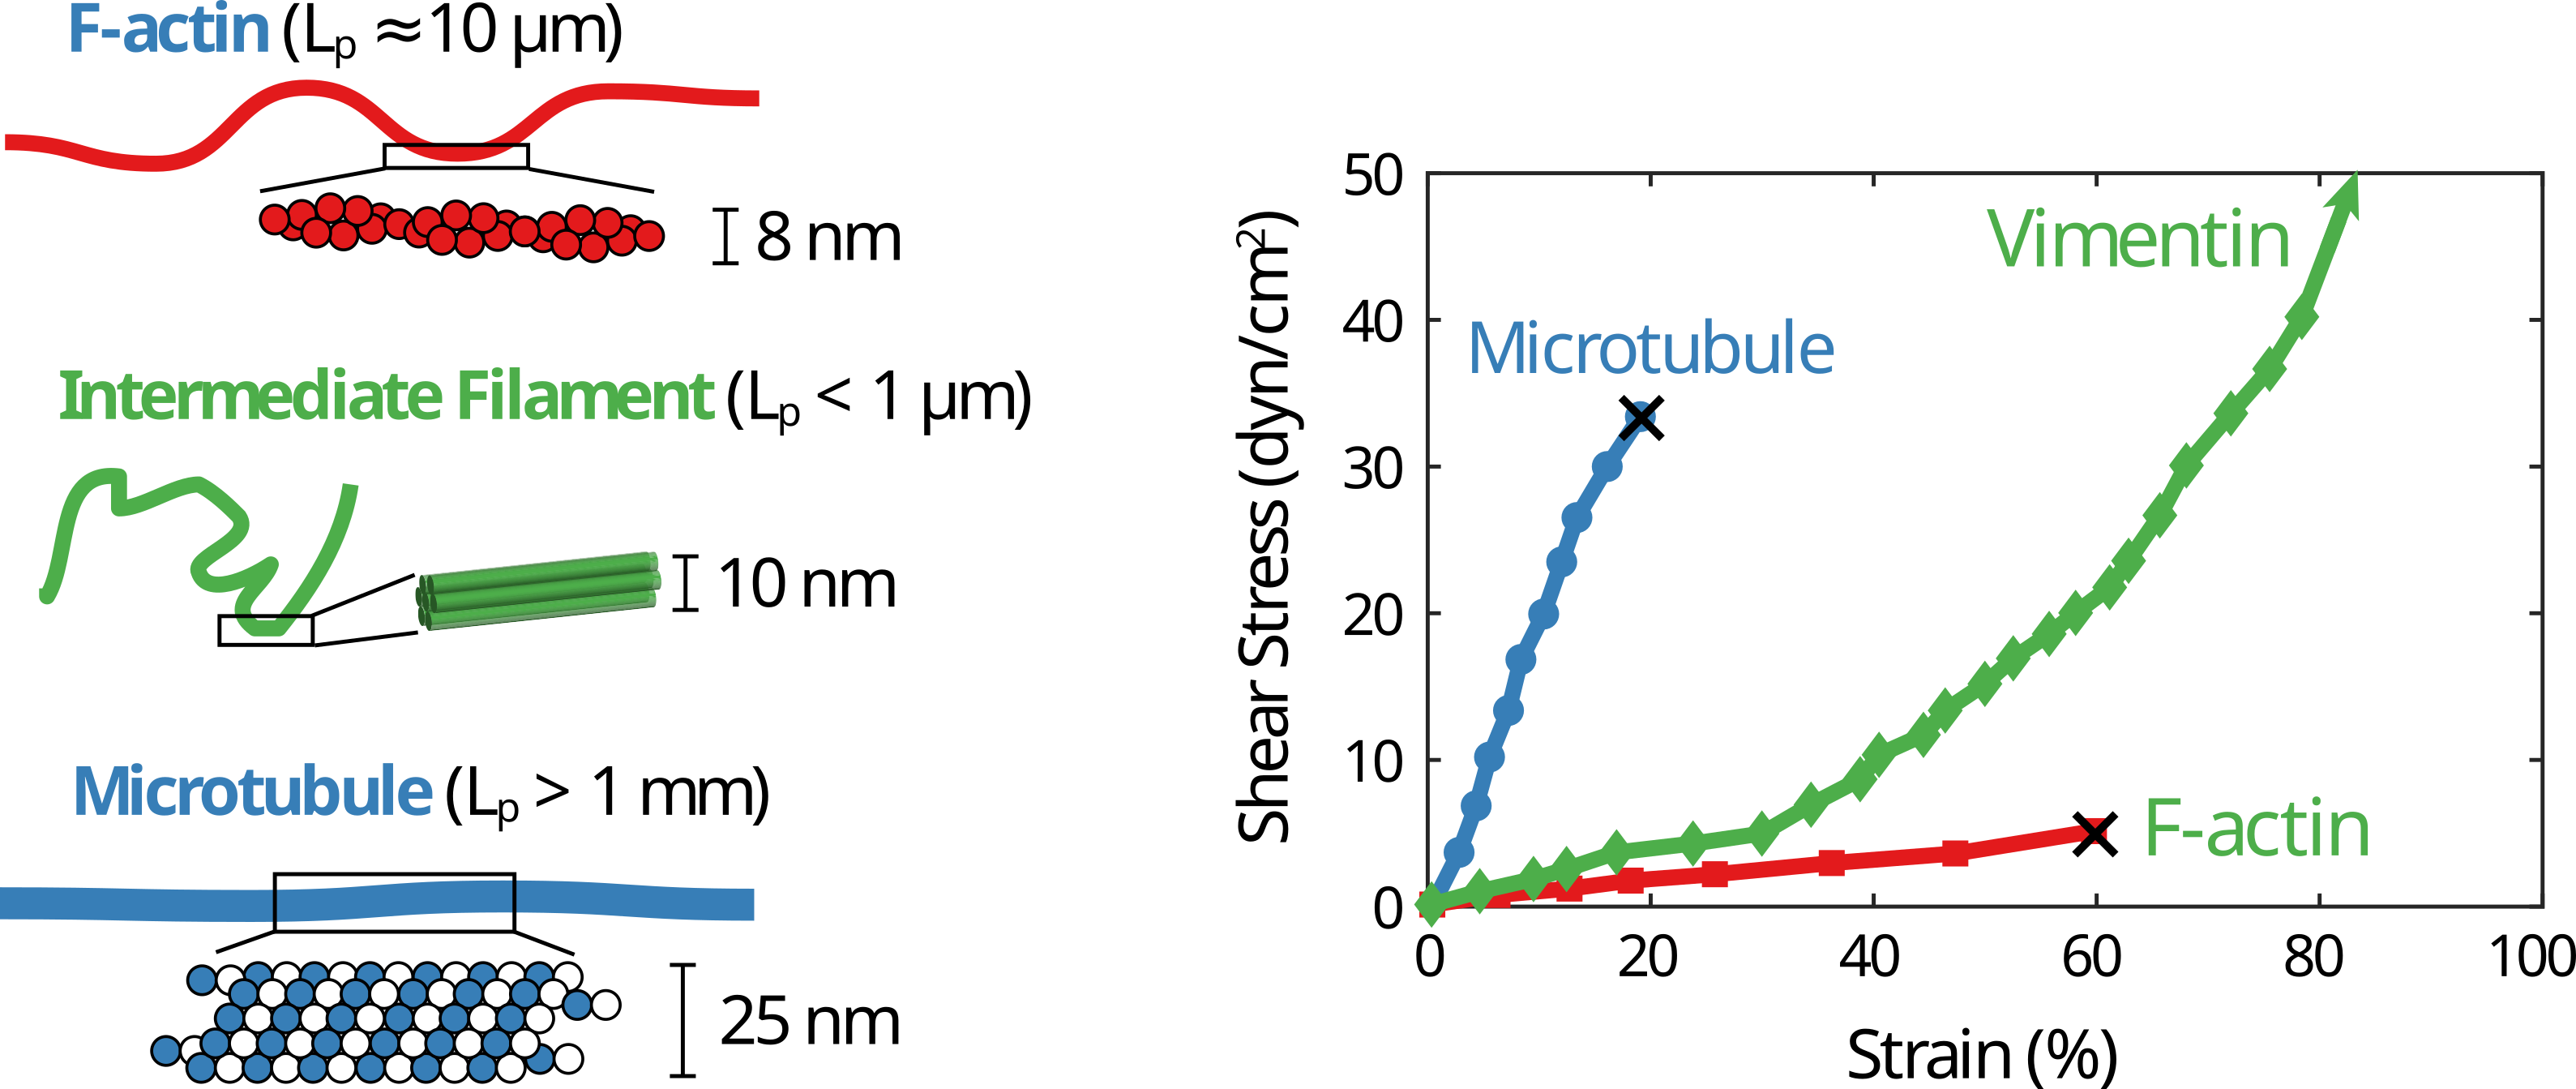
\includegraphics[width=0.8\textwidth]{chap1_filaments.png}
	\caption{\label{fig_1_3b} \textbf{Mechanics of cytoskeletal filaments}: Schematic and sizes of actin filaments, intermediate filaments and microtubules; along with the strain response to shear stress. \textit{Adapted from \cite{leggett2021}}}
\end{figure}

Multiple membrane molecules can facilitate cell adhesion, including cadherins. Cadherins are a crucial component for epithelial cell cohesion and the formation of adherens junctions, which transmit forces between cells. This key factor is involved in the mechanical regulation of cell division and tissue rearrangement during development and homeostasis \cite{godard2019, mertz2013}. Desmosomes, another type of intercellular junction, are coupled with intermediate filaments and provide mechanical resilience to cell layers \cite{hatzfeld2017, latorre2018}. Tight junctions serve as a barrier and regulate the active transport of ions across epithelial layers, playing an important role in controlling fluid pressure in tissues \cite{marchiando2010, chan2020}.

\begin{figure}[H]
	\centering
	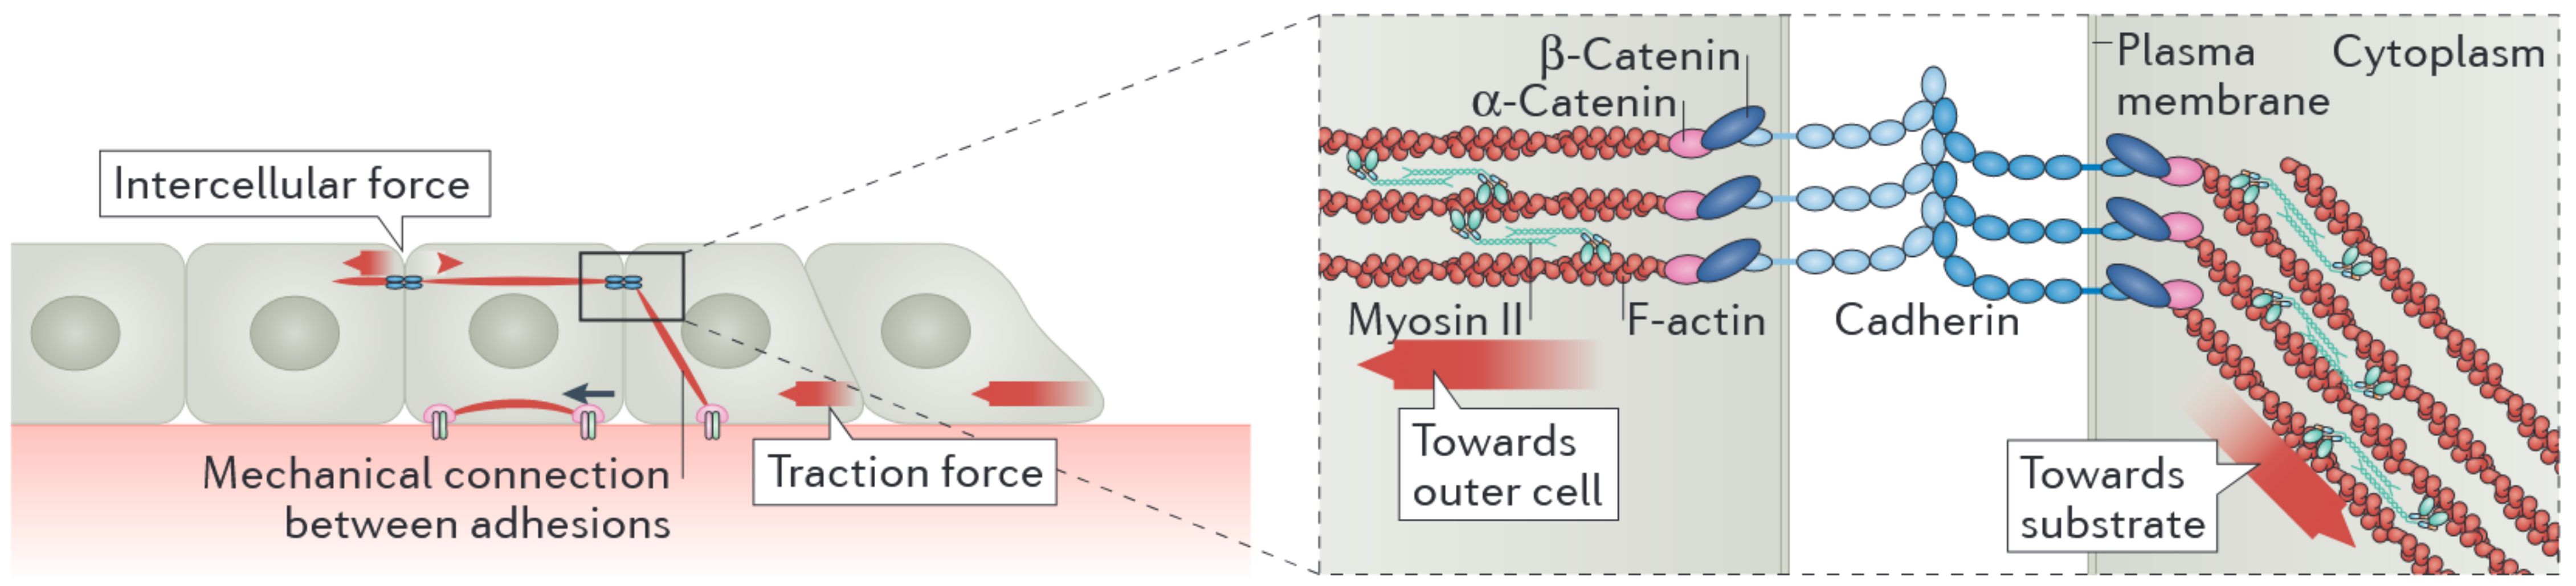
\includegraphics[width=\textwidth]{chap1_cellforces.png}
	\caption{\label{fig_1_3} \textbf{Intercellular forces through actomyosin cables and cadherins}: Schematic showing mechanical connections between adhesions and tissue force transmission with actomyosin cytoskeleton and adhesion proteins. \textit{Adapted from \cite{ladoux2017}}}
\end{figure}

\hypertarget{microenvironment}{%
	\subsection{Microenvironment}\label{microenvironment}}

The extracellular matrix (ECM) is the substrate or cell environment to which cells adhere. It is also referred to as the matrix, mesenchyme, or cellular microenvironment. The ECM serves many functions. It endows tissues with strength, thereby maintaining their shape. Additionally, it serves as a biologically active scaffolding that allows cells to migrate or adhere. The ECM also plays a role in regulating the phenotype of cells. It provides an aqueous environment that facilitates the diffusion of nutrients, ions, hormones, and metabolites between the cell and the capillary network \cite{alberts2015}.

Moreover, the ECM is subjected to mechanical forces such as blood flow in endothelia, air flow in respiratory epithelia, or hydrostatic pressure in the mammary gland and bladder \cite{waters2012, walma2020}. It has been shown that the ECM regulates cell shape, orientation, movement, and overall function in response to biophysical forces \cite{alberts2015}.

The ECM is a fibrous network of proteins, consisting of collagen, elastin, and proteoglycans as its primary structural components. Collagen is one of the most abundant proteins in the body, while elastin is the most elastic and chemically stable protein. Proteoglycans can sequester significant water as well as growth factors and proteases. The water content of the ECM allows it to deform as a poroelastic material, absorbing water upon stretching and releasing it under compression, causing a hydraulic fracture effect \cite{casares2015}. The collagen network can also remodel under the influence of cells and mechanical forces \cite{humphrey2014}.

Most ECM components undergo continuous turnover, some quickly and some slowly. For example, the half-life of collagen in the periodontal ligament is a few days, whereas that in the vasculature may be several months \cite{humphrey2014}. In response to altered physical stimuli, disease, or injury, the rates of collagen synthesis and degradation can increase many times, allowing for a rapid response.

\hypertarget{cell-matrix-interaction}{%
	\subsection{Cell-Matrix interaction}\label{cell-matrix-interaction}}

\begin{figure}
	\centering
	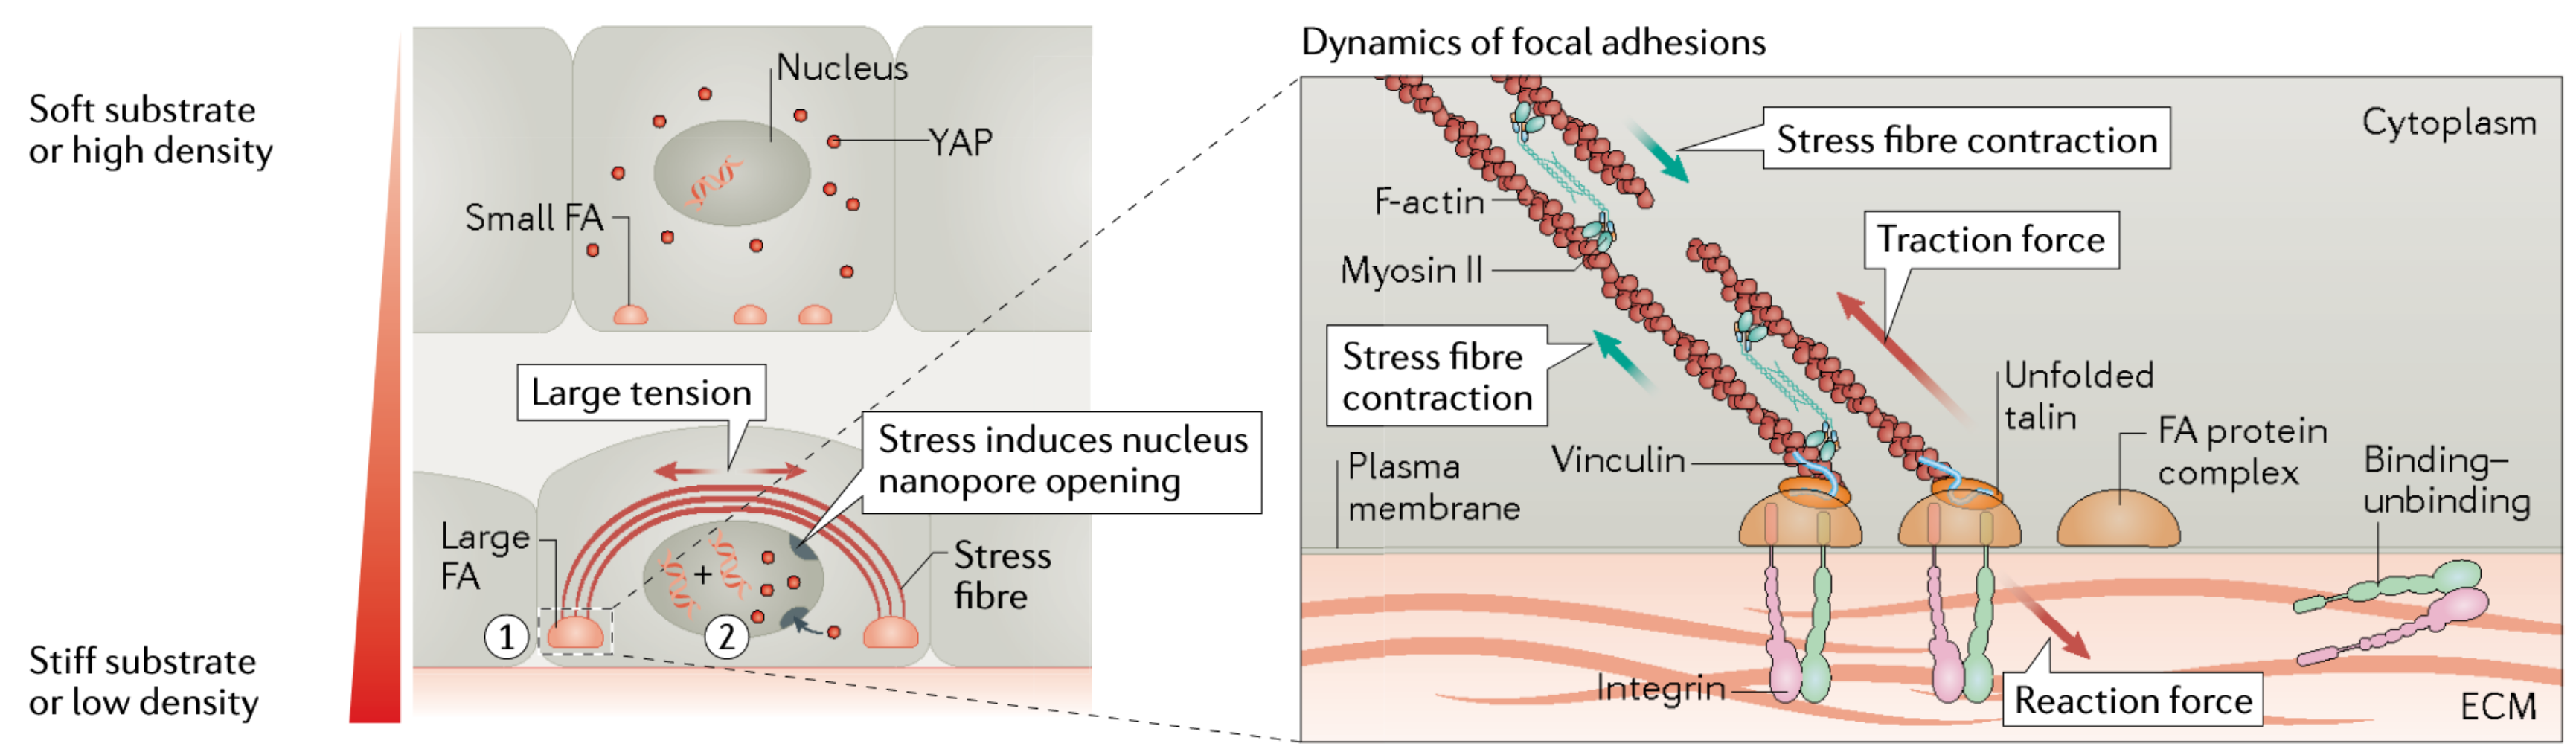
\includegraphics[width=\textwidth]{chap1_cell-matrix.png}
	\caption{\label{fig_1_4} \textbf{Cell-matrix interaction with respect to matrix stiffness and cell density}: In higher tension condition, the nucleus is deformed triggering mechanotransduction and causing alterations in cytoskeleton and tractions. \textit{Adapted from \cite{xi2018}}}
\end{figure}

The cells and the extracellular matrix (ECM) are in a dynamic relationship, constantly exchanging information and influencing each other. The cells sense the biophysical cues in the ECM through sensors such as integrins and focal adhesion complexes, which are responsible for cell-substrate adhesion \cite{kechagia2019} (see fig \ref{fig_1_4}). These adhesions allow cells to respond to various stimuli such as matrix stiffness, ligand density, and chemotactic gradients \cite{fortunato2022}. It has also been shown that cells can respond to the viscoelasticity of the matrix \cite{elosegui-artola2022}.

In addition to sensing the ECM, cells also contribute to its composition by secreting ECM components or remodeling the substrate \cite{malandrino2018}. This interplay between the cells and ECM can impact the tissue behavior fundamentally, as the connections between focal adhesions and the nucleus can affect the expression of transcriptional factors \cite{venturini2020, lomakin2020}. The precise control of cell-cell and cell-substrate interactions enables cells to transform into intricate shapes, such as curved forms in cell sheets \cite{schamberger2022}.

\hypertarget{role-in-disease-and-development}{%
	\section{Role in disease and
		development}\label{role-in-disease-and-development}}

Maintaining epithelial integrity and homeostasis is crucial for survival, and mechanisms have evolved to ensure these processes are sustained during growth and in response to damage. Epithelial cells have one of the fastest turnover rates in the body, with the entire gut cell lining turning over in 5--7 days \cite{barker2014}. This constant cell division and death pose a risk for tumor formation; it is know that 90\% of cancers emerging in simple epithelia \cite{torras2018, eisenhoffer2013}. Additionally, the high rate of cell turnover can disrupt the barrier function, as gaps should not emerge around dividing or dying cells.

If the fluid compartmentalization goes awry, it can have profound implications for epithelial and stromal homeostasis, fluid and electrolyte balance, and the development of inflammatory states. Several bacterial toxins are known to target junctions, causing changes in the tight junction protein ZO1, which compromises the barrier function and leads to pathologies such as diarrhea and colitis \cite{fasano1991}. In cancer, the compromised ZO1 barrier is essential to allow metastatic cells to break into and out of blood vessels. The leaky barrier also enables a growing epithelial tumor to access luminal fluids as an additional source of nutrients \cite{mullin2005}.

Furthermore, epithelia participate in physiological events such as epithelial--mesenchymal transition (EMT), which is a developmental process where epithelial cells gradually transform into mesenchymal-like cells by losing their epithelial functionality. EMT plays a vital role in normal biological functions such as repair and differentiation, as well as abnormal pathological activity such as organ fibrosis and promoting carcinoma progression \cite{alberts2015}. EMT endows cells with stem cell properties, enabling cell migration to distant organs and subsequent differentiation into multiple cell types during development and the initiation of metastasis \cite{thiery2009}. 

Epithelia undergo drastic shape changes with deformation and reorganization from the embryonic to the adult stage. It's not surprising that any malfunction in this process can lead to damage and disorder, resulting in congenital malformations, which are a major cause of infant mortality worldwide \cite{clarke2021}. Additionally, epithelial dysfunction is a precursor to diseases such as chronic obstructive pulmonary disease, asthma, cystic fibrosis, and pulmonary fibrosis \cite{carlier2021}.

\hypertarget{forms-of-epithelia}{%
	\section{Forms of epithelia}\label{forms-of-epithelia}}

The structure and arrangement of epithelial cells are crucial for maintaining the integrity and homeostasis of tissues and organs (see fig \ref{fig_1_5}). Simple epithelia are single-cell layers where all cells are in contact with the underlying basal lamina and have a free surface on the apical side. The shape of the cells can vary, ranging from flat to cuboidal to columnar. Stratified epithelia, on the other hand, have two or more layers of cells. Additionally, there are pseudostratified epithelia, which appear to be stratified, but are monolayers where the cell nuclei are positioned in a manner that gives the appearance of a stratified epithelium.

The classification of epithelia was first established in the XIXth century based on their structure and physiological characteristics. Germ layer theory, developed by embryologists, further expanded the epithelial nomenclature \cite{maccord2012}. During early embryogenesis, three layers emerge: endoderm, mesoderm, and ectoderm. The ectoderm forms the epithelia lining the skin, mouth, and nervous system, while the endoderm gives rise to the digestive tract, respiratory system, and liver. The mesoderm, in turn, develops the endothelia covering much of the circulatory and lymphatic systems.

It is important to note that not all tissues classified as epithelia, mentioned in this thesis, are purely composed of epithelial cells. They may be a mixture of different cell types that have epithelial-like characteristics. The focus of this thesis is on packed cell monolayers, which can form and self-organize into various 3D shapes, ranging from simple spheres to complex branched tubules. The thesis will explore the role of mechanics in epithelial morphogenesis.

\begin{figure}[H]
	\centering
	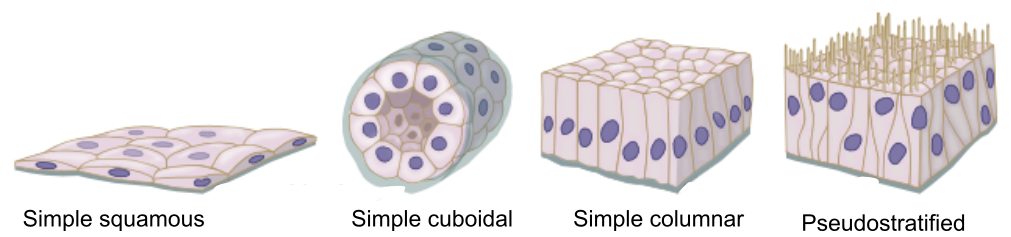
\includegraphics[width=0.75\textwidth]{chap1_forms.png}
	\caption{\label{fig_1_5} \textbf{Forms of epithelial tissues}: Simple squamous, cuboidal, columnar epithelia and pseudostratified epithelia. \textit{Adapted from \cite{zotero-9680}}}
\end{figure}


\hypertarget{the-complexity-of-the-morphogenesis}{%
\section{The complexity of the
morphogenesis}\label{the-complexity-of-the-morphogenesis}}

Epithelial cells play a crucial role in the formation of transient structures during embryonic development, such as the neural tube, somites, and precardiac epithelium, which serve as the precursor for the development of complex organs. During this process, different types of epithelia acquire distinct morphological forms and perform specific functions, including branched lungs, looped gut, kidney tubules, thyroid follicles, and sinusoids in the liver. The regulation of epithelial morphogenesis is a complex and hierarchical process that involves coordinated events at multiple spatial and temporal scales \cite{trepat2018}.

Some processes appear to be happening fast at the local level, such as cell shape changes through apical constrictions, which lead to global changes, such as the formation of a ventral furrow in a Drosophila embryo \cite{martin2009}. At the same time, chemical signaling events that activate these processes are slow and occur at a global level. The same complexity can be seen in\textit{ in vitro} systems, where a cluster of dissociated stem cells can assemble into an organoid or gastruloid and undergo global folds in response to appropriate culture conditions \cite{collinet2021}.

The underlying mechanisms of epithelial morphogenesis are intricate and involve multiple factors, including genes responding to morphogen gradients, molecular machinery involved in apical constriction, and mechanical stresses that cause tissue-scale deformations. To fully understand the phenomenon of epithelial morphogenesis, it is essential to study these processes in detail, at multiple levels of complexity \cite{schock2002, lecuit2011}.

Rudolf Virchow's third tenet of the cell theory states that ``omnis cellula e cellula,'' meaning ``all cells come from cells'' \cite{virchow1860}.
\footnote{The famous epigram was coined by François-Vincent Raspail. Virchow is regarded as influential biomedical scientist of 19th century, but more interesting part is as a radical who took part in the March revolution of 1848. He was one of the first to advocate for the social origins of illness \cite{wright2012, brown2006}.}
Although all tissues originate from cells that contain essentially the same genetic information, each tissue has a distinct architecture and function. This raises several questions, such as: what makes cells different from each other? Are differences due to genes, environmental factors, or both? What drives shape changes in tissue morphogenesis? Over the last two centuries, the field of developmental biology has addressed many of these questions, but it has also raised new issues and left others unanswered.

Until last decade, the focus of the field had been on tracking and mapping patterns of cell movements to patterns of gene or protein expression \cite{gorfinkiel2021}. While these studies are influential and important for understanding morphogenetic patterns, they fall short in explaining how cells and tissues are physically shaped \cite{veenvliet2021, odell1981}. This is because the physical understanding of tissues has been limited to kinematic descriptions, which only describe tissue deformation or cell motion. However, we know that cells and tissues actively drive shape changes and movements through the generation of mechanical forces \cite{lecuit2011}. Thus, to have an integrated understanding of morphogenesis, we must consider the role of forces and mechanics.

\hypertarget{on-growth-and-form}{%
\section{On growth and form}\label{on-growth-and-form}}

Throughout history, the form of both animate and inanimate objects has been closely linked to their intended function. In fact, the XXth century architecture principle ``Form Follows Function'' highlights the idea that the organization of a structure should be based on its intended purpose. Similarly, in developmental biology, self-assembling systems such as intestinal organoids, cancer spheroids, and gastruloids are perfect examples of this principle in action, as each structure emerges from a set of cells in a suitable environment, adapting to perform a specific biological function \cite{gjorevski2016, ishiguro2017, morizane2017, vianello2019}.

However, the opposite design principle appears to be at work in numerous \textit{in vitro} experiments that involve a controlled cellular environment. In such experiments, geometric constraints appear to drive biological function \cite{xi2018}. For instance, seeding stem cells in a bio-printed three-dimensional geometry of the gastrointestinal tract led to the production of functional tissues with physiological characteristics of
the intestine. The curvature of the structure can even control the formation of villus-like structures \cite{brassard2021}. 

\begin{figure}[h!]
	\centering
	\includegraphics[width=\textwidth]{chap2shah.png}
	\caption{\label{fig_2_1} \textbf{Multiscale imaging and tracking of embryo cell dynamics}: Top panels show in toto imaging of germlayer specification; red is mesendoderm, blue is epiblast, and yellow is endoderm. Bottom panel shows data analysis of long term pan embryo cell dynamics \cite{shah2019}}
\end{figure}

In a way, assembly of biological systems treads the line between self-organization and programmed material. Advanced microscopy techniques have allowed us to witness the intricacies of developmental processes with unprecedented clarity (see fig \ref{fig_2_1}). We can now observe cells and their motion throughout the morphogenetic process, from the formation of a spherical embryo to the creation of a complete organism \cite{shah2019}. Cells undergo shape changes and large-scale flows as they undergo morphogenesis, driven by mechanical forces in concert with biochemical processes \cite{labernadie2018, trepat2018, lecuit2011}. Thus, the dichotomy of form and function is incomplete without considering the physical laws of mechanics.


Over a century ago, D'Arcy Wentworth Thompson wrote the influential book ``On Growth and Form'' \cite{thompson1979}, in which he explored the relationship between geometry, physics, and biology in the context of morphogenesis. Thompson used examples to show how mathematical principles can explain biological phenomena, such as his theory of transformations, which demonstrates how related species can be represented geometrically (see fig \ref{fig_2_1b}). According to Thompson's daughter, he even used to draw pictures of dogs on rubber sheets and stretch them to show children how poodles could become dachshunds \cite{wolfram2022}. This distortion of shape represents significant alterations in various forces or rates of growth throughout the developmental processes of different organisms.

Thompson's approach was highly speculative, but his goal was to identify general principles behind the diverse forms and patterns found in biology. He compared growth curves of haddock, trees, and tadpoles, and found logarithmic spirals in shells, horns, and leaf arrangements.
\footnote{Funnily, He criticized the zoologists and morphologists of the time of assigning shapes to psychical instinct of the organism or some divine interference for creating the perfect shapes: “He finds a simple geometric construction, for instance in the honeycomb structure, he would fain refer it to psychical instinct or design rather than in the operation of physical forces. ... When he sees in snail, or nautilus, or tiny foraminiferal or radiolarian shell a close approach to sphere or spiral, he is prone of old habit to believe that after all it is something more than a spiral or a sphere, and that in this "something more" there lies what neither mathematics nor physics can explain}
Essentially, this book emphasized two points: first, all material forms of living things---cells, tissues, and organs---must obey the laws of physics, and second, quantitative measurements are necessary to unravel the physical principles of biology.

\begin{figure}[h!]
	\centering
	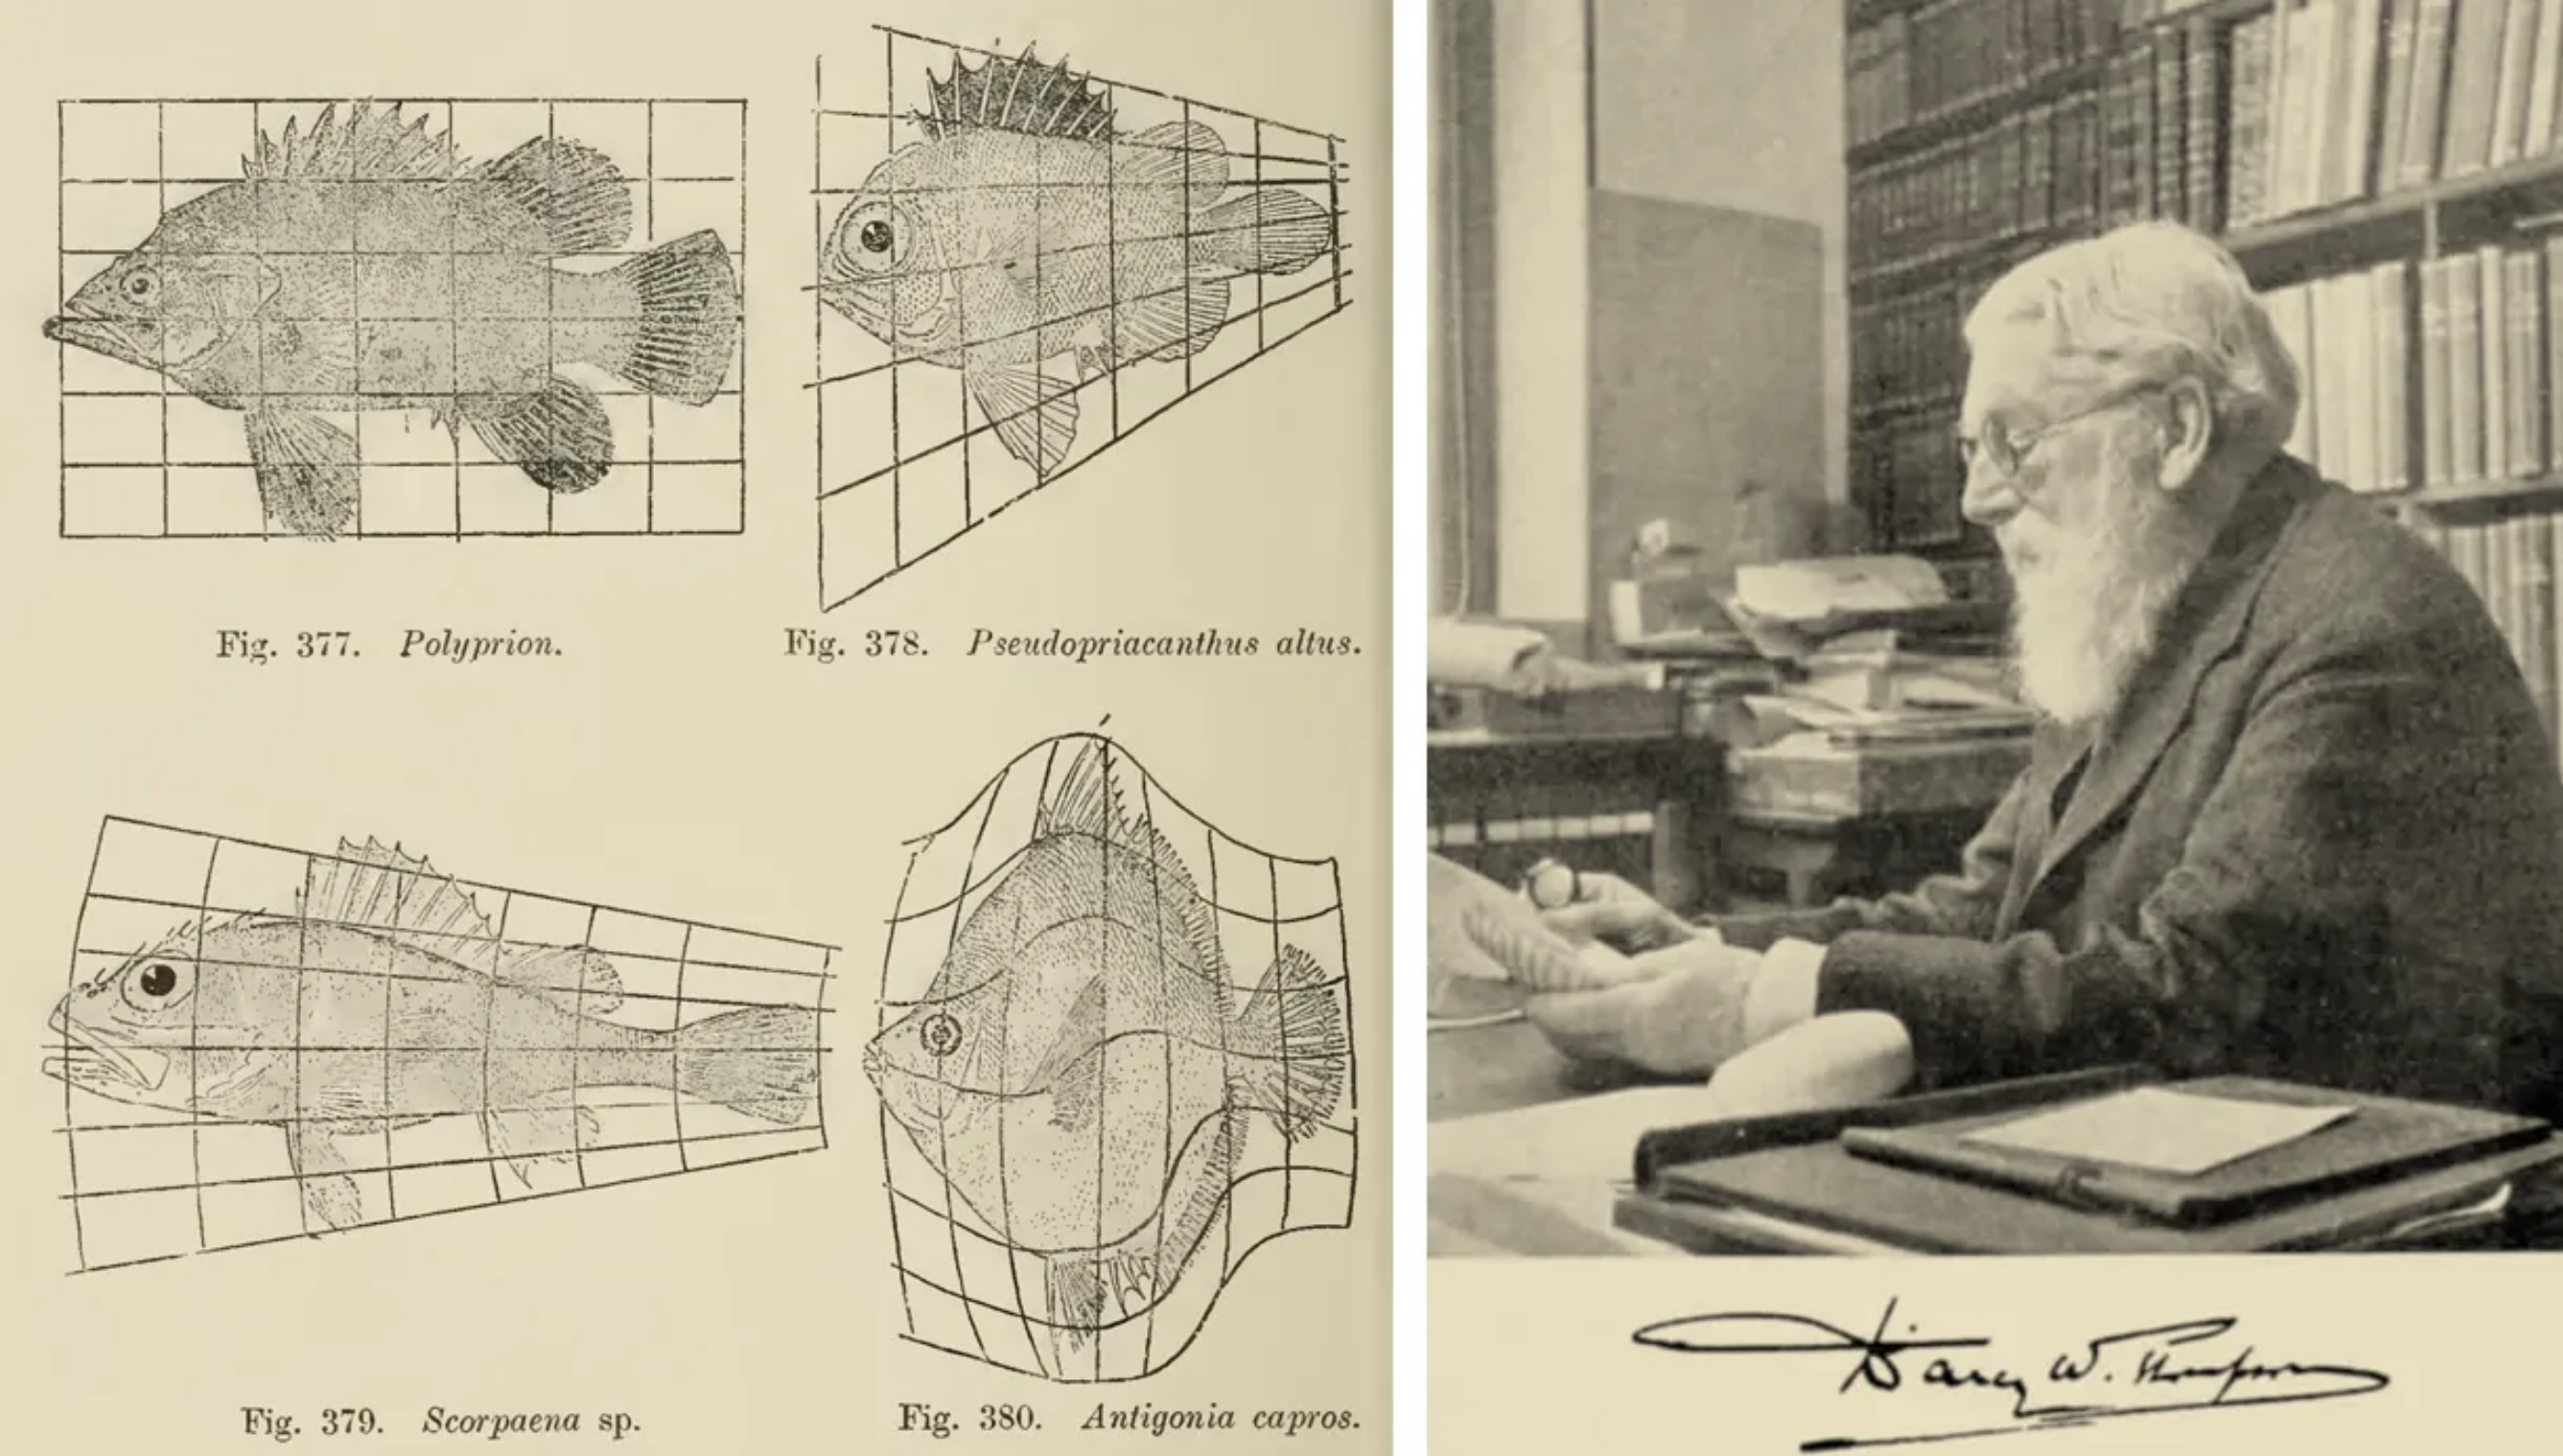
\includegraphics[width=0.75\textwidth]{chap2darcy.png}
	\caption{\label{fig_2_1b} \textbf{D'Arcy Thompson's fishes} and his theory of transformation. \cite{wolfram2017, thompson1979}}
\end{figure}

Thompson's work continues to inspire researchers even today. Right as I began my Ph.D., the centenary of the book's publication was being celebrated in the fields of developmental biology and biophysics \cite{heer2017, nat2017, natphys2017}. Even more so by the field of mechanobiology, an interdisciplinary field that studies the role of biophysical forces in cell and tissue functioning. 

\hypertarget{mechanobiology}{%
\section{Mechanobiology}\label{mechanobiology}}

The cells within epithelial tissue can be viewed as mathematical systems that integrate multiple input cues to result in an output behavior. These inputs can be mechanical or chemical, such as the stretching of lungs or the presence of morphogen gradients during embryonic development. The outputs can include cell deformation, migration, differentiation, or proliferation \cite{kumar2017}. Some outputs can even feedback into the system as an input, such as when cells remodel the matrix \cite{malandrino2018}. Mechanochemical switches at the membrane, cell-cell junctions, or cell-matrix adhesions mediate the sensing of the environment, triggering a biochemical cascade that leads to a cellular response \cite{roca-cusachs2017}. This interplay between biochemistry and mechanics is known as mechanotransduction.

During morphogenesis, mechanotransduction occurs at various scales, ranging from a single cell to complex multicellular tissue. To understand the role of different variables, experiments at different scales are necessary. It has been observed that individual cells can sense their environment and respond by altering their behavior through mechanical or biochemical processes. Whereas, multicellular systems can transmit forces and information at a longer length scale, allowing for emergent characteristics such as collective migrations, oscillations, rearrangements, and even turbulent flows \cite{heer2017, lecuit2011,trepat2018}.

An excellent demonstration of the interaction between tissues and their environment is provided by the phenomenon of durotaxis. Epithelial cells can detect changes in the stiffness of the extracellular matrix and migrate towards areas of higher rigidity. This migration towards stiffer regions has been observed both \textit{in vitro}, where cells in a monolayer collectively expand and relocate to stiffer areas, and \textit{in vivo}, such as during the migration of neural crest cells in \textit{Xenopus laevis} \cite{sunyer2016, shellard2021}. It is worth noting that the migration of neural crest cells themselves generates the durotactic gradient. In another example, during Drosophila oogenesis, the disorganized matrix is remodeled by cells to create a polarized matrix that aligns with the actin bundles in the follicular epithelium. This alignment is achieved through the coordinated rotation of cells and can guide the directed motion of cells along the polarized fibers \cite{haigo2011, cetera2014}.

The interplay between individual cells, their neighbors, and exogenous stimuli makes it difficult to decouple various biophysical aspects of the environment, such as forces, pressures, matrix stiffness, spatial confinement, porosity, or viscoelasticity. Direct force measurements in and out of tissues are also challenging. To address these challenges, researchers from various disciplines have attempted to recreate experimental systems with precise control over the biochemical and mechanical environments of cells \cite{xi2018}. This has been made possible through continuous technological advancements in fluorescent probes, imaging, microfabrication, and force measurements \cite{roca-cusachs2017}. In the following section, I will provide an overview of relevant techniques and experiments in the field of mechanobiology.

\hypertarget{synthetic-substrates}{%
\subsection{Synthetic substrates}\label{synthetic-substrates}}

The use of Polyacrylamide and soft PDMS gels has enabled researchers to investigate mechanical interactions at cell-substrate adhesion (see fig \ref{fig_2_2} A). Simply seeding cells on hydrogels of different stiffnesses reveals a significant impact on the actin cytoskeleton, cell shape, and lineage specification \cite{yeung2005,  engler2006}. These substrates, because of their known elastic response, are also utilized in techniques like traction force microscopy (TFM) to measure the forces exerted by cells and tissues on the substrate \cite{harris1980,  gomez-gonzalez2020} (see fig \ref{fig_2_2} D). TFM studies have shown that cells and tissues can exert greater forces on stiffer substrates as a result of the remodeling of the cytoskeleton \cite{elosegui-artola2016}. Higher matrix stiffness has also been found to induce the translocation of Yes-associated protein (YAP) from the cytoplasm to the nucleus, which is considered a sensor for mechanotransduction \cite{elosegui-artola2017}. However, increasing extracellular matrix (ECM) ligand density alone can induce YAP nuclear translocation without changing substrate stiffness \cite{stanton2019}.

\hypertarget{geometric-control}{%
\subsection{Geometric control}\label{geometric-control}}

The shape of cells or tissues on 2D substrates can be controlled using micropatterned adhesion proteins or microfabricated stencils. Protein patterning techniques are used to pattern adhesion promoting proteins and control cell attachment and spreading, while microfabricated stencils physically confine cells in a particular geometry (see fig \ref{fig_2_2} B C). When cells are confined, they respond by reorganizing their actin cytoskeleton and focal adhesion complexes to match the shape imposed on them \cite{vignaud2012}. Confined tissues undergo larger-scale rearrangements, leading to the formation of fascinating topological defects or oscillations \cite{tlili2018,  balasubramaniam2021,  guillamat2022}. Through these experiments, we can uncover the mechanisms of force transmission and regulation of collective cell migration and epithelial growth in two dimensions \cite{nelson2005,  vedula2012,  deforet2014}.

Embryonic stem cells subjected to 2D confinement have been shown to differentiate based on the shape and size of the confinement. For example, a circular monolayer of stem cells can reproduce the tissue patterning of a 3D gastruloid \cite{warmflash2014}, and confinement in a triangular shape can lead to high tension at the vertices and activate Wnt signaling, promoting differentiation to mesoderm \cite{muncie2020}. Moreover, advancements in photopatterning technologies allow for precise control of multiple proteins on the same substrate \cite{guyon2021, prahl2022}, enabling the establishment of complex co-culture systems that mimic \textit{in vivo} events.

Not just 2D shape, epithelial monolayers are also able to respond to curvature by regulating cell migration, orientation, cell/nucleus size, and shape \cite{marin-llaurado2022, schamberger2022} (see fig \ref{fig_2_2} C). For example, an epithelial monolayer on hemispheres of elastomers acts as a fluid with increasing curvature \cite{tang2022}. On a smaller scale, cells attached to corrugated hydrogels show variations in lamins, chromatin condensation, and cell proliferation rate in response to curvature \cite{luciano2021}. Bio-printing of three-dimensional tissue architectures can also create functional tissues \cite{brassard2021,  breau2022}.

\begin{figure}[h!]
	\centering
	\includegraphics[width=\textwidth]{chap2mechnobiology.png}
	\caption{\label{fig_2_2} \textbf{Mechanobiological strategies for studying morphogenesis} \textit{Adapted from \cite{vianello2019}}}
\end{figure}

\hypertarget{mechanical-control}{%
\subsection{Mechanical control}\label{mechanical-control}}

Living systems have mechanical control in addition to spatial control, as physical forces emerge from growth, deformation, and remodeling of the extracellular matrix (ECM) and fluid pressure in closed geometries. For example, the intestinal epithelia are stretched during peristaltic movements in the gut and lung alveoli deformations during breathing. Compression can also guide morphogenetic events that involve tissue bending and folding, such as the formation of the optic cup, gut villi, and cortical convolutions in the brain \cite{okuda2018, shyer2013, tallinen2016}.

To study tissue behavior under external perturbation, cells and tissues are probed at the molecular and subcellular scales using techniques such as atomic force microscopy, magnetic beads, optical tweezers, and micropipettes \cite{bao2003} (see fig \ref{fig_2_2} E). At a larger scale, various types of stretching devices, tissue rheometers, and force plates can be used \cite{xi2018}. These experiments reveal that cells exhibit complex viscoelastic behavior at different levels of deformation and different regions of the cytoskeleton \cite{mofrad2009}. The response of tissues to stretching can vary depending on the timescale of the stretch and the reorganization of
cells within the tissue \cite{guillot2013}. Rheological experiments also help to uncover the role of signaling pathways, such as YAP transcription factors, in mechanosensation \cite{wagh2021}.

The microfluidic system, also known as ``cells on a chip,'' has emerged as a valuable tool for investigating cell behavior under controlled biophysical conditions that mimic \textit{in vivo} conditions \cite{ingber2018}. This
system allows for the application of stretch or shear forces, as well as the creation of a controlled microenvironment that mimics the organ-level cues present in the body. For instance, the surface tension at the air-liquid interface in the lungs and the fluid flow through the vasculature, as well as the cyclic mechanical stretch of the tissue-tissue interface due to breathing, can be replicated using this approach \cite{huh2010}.

In the context of developmental biology, the use of microfluidic systems has allowed for the study of self-organization and embryo functions under controlled physical conditions. The co-culture of iPSC-derived motoneurons and brain microvascular endothelial cells in a microfluidic system has produced the \textit{in vivo}-like maturation of spinal cord neural tissue, representing a new avenue for exploring the complex interplay between physical and biological factors in development \cite{sances2018, samal2019}.

As mentioned earlier, the tissue-matrix interaction plays a critical role in sensing and rapidly transmitting forces \cite{tambe2011, sunyer2016, serra-picamal2012}. However, in early embryonic epithelia where little or no ECM is present, stresses generated by actomyosin contraction of the cells in one tissue are transmitted over long ranges via intercellular adhesions to other tissues. Thus, studying a simple free-standing epithelial monolayer is very appealing in terms of characterizing the mechanical response to stretch at different time scales.

Only two techniques are available for this: first, Harris and colleagues created a suspended monolayer by culturing a cell monolayer on a collagen matrix on two rods, and later removed the matrix using enzymatic digestion \cite{harris2012}. Second, epithelial domes, where MDCK cells pump ions to form fluid-filled blisters, have been used \cite{lever1979}. Recently, my colleagues, Ernest Latorre and Ariadna Marin-Llaurado, have enhanced control over the curvature, shape, and size of the domes \cite{latorre2018, marin-llaurado2022}, details on this system in the next chapter. These experiments showed that elasticity measurements of the monolayer were two orders of magnitude larger than those of individual cellular parts, and the monolayer could sustain more than 200\% strain before the rupture of cell-cell junctions. The cell cytoskeleton, particularly the actomyosin network and cadherin junctions, actively remodel during stretching, while the keratin network reinforces monolayer integrity at higher strains \cite{latorre2018, duque2023}. With sustained stretching, the tissue undergoes significant realignment and rearrangement via division \cite{wyatt2015}. Experiments on tissue devoid of the matrix also revealed epithelial actions such as superelasticity and buckling \cite{latorre2018, wyatt2020}.

\hypertarget{d-systems}{%
\subsection{3D systems}\label{d-systems}}

\textit{In vitro} experiments with 2D or 2.5D cell systems have improved our understanding of cell mechanics in morphogenesis by allowing us to measure deformations and forces and control environmental conditions that are inaccessible \textit{in vivo}. However, to gain a deeper understanding of cell mechanics, systems closer to the \textit{in vivo} environment must be probed.

Cell aggregates are a promising \textit{in vitro} system for probing cell mechanics, where synthetic matrix and mechanical measurement tools can be used. The response of cell clusters to the matrix, while similar to planar tissues, is more complex and includes sensitivity to matrix stiffness, confinement, and ECM concentration, as well as the ability to undergo 3D shape transformations (see fig \ref{fig_2_2} E). Our lab has demonstrated that cell aggregates perform durotaxis and exhibit wetting behavior dependent on stiffness \cite{perez-gonzalez2019, pallares2022}. Additionally, cell aggregates in suspension behave like viscous droplets and can be used to measure rheological properties, such as when squeezed between plates or probed with AFM or a micropipette \cite{xi2018}. The viscoelastic properties of cell aggregates can even be measured by coalescing two aggregates
\cite{oriola2022}.

In recent years, the use of hydrogel systems for the culturing cell aggregates has gained significant attention. Hydrogels, such as polyethylene glycol (PEG), polyacrylamide, collagen, or Matrigel, serve as a supportive environment for cell growth. Naturally extracted hydrogels like Matrigel provide a similar architecture to the native ECM. When embedded into a hydrogel, polarized epithelia tend to form a spherical structure with a hollow lumen, which can be induced to form branching morphogenesis by hepatocyte growth factor \cite{bryant2008}. 

Cell-driven self-assembly in organoids leads to tissue formation that mimics organ features, but achieving reproducibility in shape and composition is often challenging \cite{nelson2008, hofer2021}. Synthetic hydrogels with control over ligand presentation, crosslinking, and degradability have proven useful for epithelial organoids, allowing for control over cell fate \cite{gjorevski2016, gjorevski2022}.

3D gel-based culture systems with spatiotemporal control over the mechanical properties corresponding to \textit{in vivo}-like functional structures have also been developed \cite{torras2018}. Interestingly, recent publications show tissue transformation from planar to complex organ-resembling tissue without fine environmental control. For example, intestinal epithelium mechanically compartmentalizes itself, and 2D stem cells transform into a 3D neural tube \cite{perez-gonzalez2021, karzbrun2021}.

In developing embryos, both embryonic and extraembryonic fluids generate frictional and tensional stresses when flowing, or hydrostatic pressures when confined within spaces \cite{vianello2019, chan2020}. The challenge of measuring these forces has led to the use of various techniques, including micropipette aspiration. Micropipette experiments, where a needle is inserted into the embryo to control pressure, have revealed that the internal hydrostatic pressure determines the embryonic size and dictates cell fate allocation \cite{chan2019} (see fig \ref{fig_2_2} E). As a fluid-filled structure, the hydrostatic pressure inside the embryo corresponds to tension in its surfaces, and changes in luminal volumes are sensed by cells through increased cortical tension, inducing changes in cell shape and cytoskeleton organization \cite{chan2019, choudhury2022}. Micropipette aspiration has also been effective in measuring the surface tension of individual cells or whole blastomeres \cite{dumortier2019}, thus providing insight into the role of the actin cortex in regulating preimplantation embryonic contractility \cite{ozguc2022, firmin2022}.

The measurement of forces within embryos has also been approached through the insertion of deformable probes, such as hydrogels, oil, or magnetic droplets \cite{dolega2017, campas2014, serwane2017}. The shape changes of these probes allow for measurement of local forces and osmotic pressures \cite{mongera2023}.

In addition to embryos, explant systems have been utilized to study organogenesis in the brain, gut, and lungs. Lung explant research has been particularly useful in understanding different aspects of shape formation, which occurs under the influence of pressure and growth factors. The explant system allows for direct control over the chemical and mechanical environment at specific stages of development. Work with mouse airway epithelium has shown that pressure and matrix stiffness impact the number of lung branches \cite{palmer2021, varner2015, nelson2017}.

Other tools such as optical tweezers, laser ablation, and optogenetic excitations have been used at different levels to probe the mechanics of development \cite{lecuit2011, gomez-gonzalez2020}. However, independent control over multiple factors remains difficult and force measurement remains indirect.

In conclusion, epithelial tissues are highly sensitive to various biophysical forces and constantly undergo remodeling at different scales and timeframes. There are multiple techniques available to manipulate and study these tissues, from single cells to embryos, with controlled forces and deformation. Due to its dynamic behavior, epithelial tissue can be considered an active material. The focus of this thesis is to develop a system that can control and measure physical forces to understand epithelial behavior as an active material. In the following chapter, we will delve into the molecular machinery responsible for driving these active tissues.

\chapter{Active tissue mechanics}
\chapter{Bottom-up biology}

\part{Results}
\chapter{Novel microfluidic system for generating 3D epithelia with controlled pressure and shape}
\chapter{Epithelial stretching is driven by viscoelasticity of actomyosin cortex}
\chapter{Epithelial buckling produces predictable folds}

\part{Conclusions and Discussion}
\chapter{Conclusions and Discussion}
\section{Developed a novel device to create 3D pressure controlled epithelia}
\section{Actin cortex drives epithelial tissue stretching}
\section{Rapid deflation leads to buckling}
\section{Controlling 3D patterns of epithelial sheets}

%now enable appendix numbering format and include any appendices
\begin{appendices}
	\chapter{Methods}
	\hypertarget{creating-pressurized-epithelia}{%
	\section{Creating pressurized
		epithelia}\label{creating-pressurized-epithelia}}

\hypertarget{fabrication-of-microfluidic-devices.}{%
	\subsection{Fabrication of microfluidic
		devices.}\label{fabrication-of-microfluidic-devices.}}

Polydimethylsiloxane (PDMS) gels (Sylgard PDMS kit, Dow Corning) were
used to make the microfluidic devices. PDMS was synthesized by mixing
the curing agent and elastomer in 1:9 weight ratio. This mixture was
centrifuged for 2 min at 900 rpm to remove air bubbles. The
unpolymerized PDMS was poured into a mold or spun to obtain the desired
shape. There are four parts to the device (fig S1X showing device
scheme). First is the top block, a thick PDMS block with four inlets and
one channel for the application of hydraulic pressure. The second is a
200 um thin PDMS layer with a 1.2 mm diameter hole in the center with a
400 nm porous membrane (Polycarbonate filtration membrane 0.4 um,
Whatman membranes) attached to it. The third is another 200 um thin PDMS
layer with a channel for seeding the cells. Lastly, all these PDMS parts
are attached to, the fourth part, a glass-bottomed 35 mm dish (35 mm,
no. 0 coverslip thickness, Cellvis). The top block was made using
replica molding in a 3D printed mold. This mold was 3D printed with vat
polymerization and a digital light processing 3D printer (Solus DLP 3D
Printer with SolusProto resin). The mold's surface was then silanized
using Trichlorosilane (Trichloro(1H,1H,2H,2H-perfluorooctyl) silane,
Merck) for preventing adhesion with unpolymerized PDMS. PDMS was poured
into the mold and degassed for one hour. PDMS is cured with a hot plate
at 100 C for 30 min. Once cured, PDMS is removed, cut into devices, and
punched with 1.5 mm. 200 um thin PDMS layers were made by spin coating
4.5 ml unpolymerized PDMS on a 15 cm dish at 500 rpm for 1 min. These
dishes were incubated in an oven at 80 C to polymerize for 12 hr. These
thin sheets were cut into the parts of devices using a Silhouette
cutting machine (Silhouette Cameo 4, Silhouette America). The sheets
were attached to a Silhouette cutting mat and then Silhouette software
was fed with the pattern of the device layers. A sharp cutting tool in
the machine cut the PDMS along the pattern. These cut PDMS were peeled
off with help of 70\% ethanol. These devices are assembled with the aid
of ozone plasma cleaner (PCD-002-CE, Harrick Plasma). Glass bottomed
dishes and thin PDMS layers with cell channels were treated for 1 min
under plasma. Then bonded together by placing the layers in contact for
2 hr at 80 C. Similarly, the top block and thin membrane with porous
membrane were also bonded. These layers were later bonded together again
using plasma cleaner.

\hypertarget{patterning-protein-on-the-device}{%
	\subsection{Patterning protein on the
		device}\label{patterning-protein-on-the-device}}

The devices were filled with 96\% ethanol for removing air bubbles.
Then, devices are treated with 5\% v/v (3-aminopropyl) triethoxysilane
(Merck) diluted in 96\% ethanol for 3 min and rinse three times with
96\% ethanol. Later the devices were filled with MilliQ water to remove
ethanol traces. PRIMO (Alveole Lab) was used to pattern
adhesion-promoting protein. For this setup, devices were incubated with
PLL (Poly-L-lysine solution, Merck) for 1 hr, subsequently with SVA PEG
(50mg/ml in 8.24 pH HEPES) for 30 min, and rinsed with HEPES. Before
using PRIMO, devices were filled with a photoinitiator. Desired protein
pattern was loaded into the PRIMO software (Leonardo, Alveole Lab).
PRIMO uses a microscope to shine the laser in the specific region
according to the loaded pattern to cut PEG chains. Samples were rinsed
with phosphate-buffered saline (PBS, Merck). Then the samples were
filled with fibronectin and fibrinogen (100 ug/ml Fibronectin in 2\%
Far-red fibrinogen solution in 1X PBS) solution for 5 min. Then samples
were rinsed again with 1X PBS. Fibrinogen labels the fibronectin with
Far-red signal to image the coated protein pattern.

\hypertarget{cell-culture-in-the-device}{%
	\subsection{Cell culture in the
		device}\label{cell-culture-in-the-device}}

To image cell shape and tissue structure Madin-Darby Canine Kidney
(MDCK) cells expressing CIBN-GFP-CAAX were used for the experiments.
CIBN-GFP-CAAX labels plasma membrane. These cells were cultured in
Dulbecco's Modified Eagle Medium (DMEM, Gibco Thermofisher) with 10\%
v/v fetal bovine serum (FBS, Gibco, Thermofisher), L-glutamine
(Thermofisher), 100 ug/ml streptomycin and penicillin. Cells were
incubated at 37 C with a 5\% CO2 condition. Before seeding cells in the
device, it is filled with a cell culture medium. Cells are trypsinized
and diluted at a concentration of 25x106 cells/ml. The cell channel of
the device is filled with 30 ul of cell solution and incubated for cell
adhesion. After one hour of incubation, devices are rinsed with media to
remove unattached cells. Devices were kept 24 hr in the incubation for
the growth of a monolayer before the experiment.

\hypertarget{application-and-measurement-of-the-pressure}{%
	\subsection{Application and measurement of the
		pressure}\label{application-and-measurement-of-the-pressure}}

The pressure is applied via hydrostatic forces similar to the previous
studies {[}Choudhury2022 Piotrowski2017 Palmer2021{]}. The two channels
in the chip were separated by the porous membrane. Cells are on the
bottom side of the membrane. The pressure in the channel (top side of
the membrane) is used to inflate the structures on the top. This channel
has one inlet and one outlet for removing bubbles. The inlet is
connected to a 35 ml reservoir of cell culture medium (in a 50 ml falcon
tube) by tubing (PTFE Tubing 1/16'' OD for Microfluidics, Darwin
microfluidics) and the outlet is connected to a shutoff valve
(Microfluidic Sample Injection / Shut-off Valve, Darwin microfluidics).
Once bubbles are removed, closing the valve would apply the pressure on
the basal side of the cells according to the difference between the
height of the fluid level. All tubings are connected to the chip with a
steel insert (Stainless steel 90° Bent PDMS Couplers, Darwin
microfluidics). We are able to find zero by matching the height of the
device to the liquid and air interface in the reservoir. This is
confirmed with the experiments, where on applying pressure domes form
but on reduction in pressure to zero domes deflate.

\hypertarget{confocal-microscopy}{%
	\subsection{Confocal Microscopy}\label{confocal-microscopy}}

For timelapse imaging of domes at a larger time interval (\textgreater{}
1 min), an inverted Nikon microscope with a spinning disk confocal unit
(CSU-W1, Yokogawa) was used with Nikon 40x, 20x, and 10x air lenses. For
shorter time intervals (\textless{} 10 s), a Zeiss LSM880 inverted
confocal microscope was used with laser scanning mode. Fast imaging was
enabled by imaging a single line in the middle of the dome.

\hypertarget{fabrication-method-for-the-light-sheet-device}{%
	\subsection{Fabrication method for the Light-Sheet
		device}\label{fabrication-method-for-the-light-sheet-device}}

The devices used with the light-sheet microscope consisted of a single
PDMS block bonded to a glass microscope slide (76x26 mm, RS Components
BPB016). The blocks were made using a 3D printed mold (Ultimaker 3 with
Ultimaker PLA Printer Filament 1616). PDMS was mixed, centrifuged,
degassed, and cured as described above for the normal devices. Once
cured, the PDMS was removed, cut into individual devices and punched
with a 1.5mm biopsy punch. The PDMS blocks were then attached glass
slides using a thin layer of unpolymerized PDMS, that was coated onto
the glass slides using a spatula. The devices were then kept on a
hotplate at 100C for 30mins to allow the PDMS bonding to fully cure. The
400nm porous membranes were then attached to the devices. The edges of
the membrane were carefully dipped into unpolymerized PDMS, before being
placed flat on the top of the device. Particular care was taken to
ensure the centre of the membrane over the punched pressure-application
hole remained free of PDMS. The devices were then kept at 65C for 1 hour
to allow the PDMS bonding to fully cure.

\hypertarget{device-protein-patterning-and-cell-culture-in-light-sheet-device}{%
	\subsection{Device protein patterning and cell culture in Light-Sheet
		device}\label{device-protein-patterning-and-cell-culture-in-light-sheet-device}}

The light-sheet devices were protein patterned and cell cultured using
the same methods and steps as outlined above for the normal devices,
with the one minor addition of the use of a simple PDMS and glass cap
for a few critical steps. The porous membrane for pressure application,
and thus the site of protein patterning and cell seeding, for the
light-sheet devices is exposed and on the top side of the devices. This
mostly allowed for easy application of reagents as a droplet could be
applied and aspirated directly, however for the more sensitive steps in
the procedure, a simple PDMS and glass device was used to create a
temporary covered channel over the porous membrane to regulate the
procedure and ensure the treatment of the devices was highly
standardised. Specifically, the cap was used for the application of
photoinhibitor during PRIMO, and for the application of cell solution
during cell attachment. The caps were fabricated using 2cm x 2cm squares
of a 400µm thick PDMS layer, with a keyhole shape cut in from the side.
Each PDMS piece was then stuck to a 18mm diameter coverslip (18mm, no.1
Cover glasses circular, Marienfeld 0111580) using the innate attraction
between the surfaces.

\hypertarget{application-and-measurement-of-pressure}{%
	\subsection{Application and measurement of
		pressure}\label{application-and-measurement-of-pressure}}

The experimental apparatus and measurements for the light-sheet devices
were the same as the normal devices as outlined above. Light-sheet
microscopy The imaging of the light-sheet devices was done with a
dual-illumination inverted Selective Plane Illumination Microscope
(diSPIM) (QuVi SPIM, Luxendo, Brucker) with Nikon 40x immersion lenses
(Nikon CFI Apo 40x W 0.8 NA NIR water immersion objective). For the
buckling experiments, only single objective illumination and detection
was used.

\hypertarget{quantitative-analysis-of-the-domes}{%
	\section{Quantitative analysis of the
		domes}\label{quantitative-analysis-of-the-domes}}

\hypertarget{quantification-of-the-dome-areal-strain-and-tension}{%
	\subsection{Quantification of the dome areal strain and
		tension}\label{quantification-of-the-dome-areal-strain-and-tension}}

As mentioned earlier, the domes were imaged in 3D with confocal
microscopy. We used ImageJ to manually section the dome in the middle in
the YZ plane, XZ plane is a plane parallel to the monolayer, with
Reslice function along the Z axis. This section was used to calculate
the height, radius of curvature, and base radius. Strain was calculated
as {[}Strain = height2/base2{]} and tension as {[}Sigma = 0.5PR{]}. The
raw data was extracted in ImageJ and then MATLAB was used to compute and
plot the strain and tension.

\hypertarget{analysis-of-the-kymographs}{%
	\subsection{Analysis of the
		kymographs}\label{analysis-of-the-kymographs}}

For cyclic pressure or buckling experiments, the domes were imaged at
low resolution and high noise levels to capture fast dynamics. The
previous method of manually quantifying each time point is not feasible.
Thus, we used the ImageJ function of the Reslice function along the time
axis. We resliced it along the Y-time axis in the middle of the dome,
such that we get a kymograph of height as a function of time. Also, we
performed the reslicing along the XT axis at the plane of the monolayer,
such that we get the kymograph of the base radius with respect to time.
These kymographs were in form of images save manually with ImageJ. A
custom-built MATLAB code was used to digitize the kymographs, where
maximum intensity along each time was considered as the current dome
height position. The first 30 s of the experiment pressure is zero, so
the unstretched monolayer position is determined fom those time points.
Dome height is calculated with the difference between the current
position and the initial position. Base radius is calculated similarly
by subtracting two sdes. The radius of curvature is calculated using the
relation between the base and height of the dome. {[}R = h2+a2/ 2h{]}

\hypertarget{qualitative-analysis-of-the-buckling-event}{%
	\subsection{Qualitative analysis of the buckling
		event}\label{qualitative-analysis-of-the-buckling-event}}

Whether domes are buckling or not was determined manually checking every
frame during the deflation. If dome maintains the smooth circular
geometry in XZ plane during the deflation, we mark the dome as ``not
buckling''. However, if the dome has a visual discontinuity in the
curvature or a kink it is then considered to be ``buckling''. Imaging
the fast events in XY plane was done in an ad hoc manner. To capture the
folds, the dome as imaged closer to the apical surface of the monolayer.
The type of fold was determined by carefully observing the way which
monolayer makes contact with the imaging plane. If there is one point of
contact in the centre and spreads outwards, it is considered as
accumulation along the periphery. In case where there are multiple
points of contact and they all join in the middle, it is considered as a
network of folds.

	\chapter{Detailed protocols}
	\chapter{Codes}
	\chapter{Funding}
\end{appendices}

%next line adds the Bibliography to the contents page
\addcontentsline{toc}{chapter}{Bibliography}
%uncomment next line to change bibliography name to references
%\renewcommand{\bibname}{References}
\bibliography{refs}        %use a bibtex bibliography file refs.bib
%\bibliographystyle{plain}  %use the plain bibliography style

\end{document}

